% ==============================================================================
% CHAPTER 2: FROZEN REGIME FOUNDATIONS
% ==============================================================================
% Content ported from Paper 2 (DOI: 10.5281/zenodo.18211854)
% Framework 2.0 language wrappers added; math content verbatim
% ==============================================================================

% ------------------------------------------------------------------------------
% 2.1 READER MAP
% ------------------------------------------------------------------------------
\section{Reader Map}
\label{sec:ch2_reader_map}

\begin{tcolorbox}[colback=blue!3!white, colframe=blue!50!black,
    title=\textbf{Framework 2.0 Reminder}]
\textbf{EDC Projection Principle:} Every physical process has a \textbf{5D bulk+brane cause}
whose observable residue is a \textbf{3D shadow} on the observer boundary.

In this chapter:
\begin{itemize}[nosep]
    \item \textbf{5D cause:} Membrane tension $\sigma$, topological defect structure, frozen vs.\ fluid regimes
    \item \textbf{Brane process:} Step-function profiles, energy minimization, isoperimetric/Steiner constraints
    \item \textbf{3D shadow:} Electron mass, proton mass, fine-structure constant $\alpha$
\end{itemize}
\end{tcolorbox}

\subsection{What This Chapter Proves}

This chapter establishes the \textbf{mathematical foundations} that the rest of Part II depends upon.
The key results are:

\begin{enumerate}
    \item \textbf{Frozen vs.\ Fluid:} Why Ginzburg-Landau (GL) smooth profiles \emph{fail} (598\% error)
          while frozen step-function profiles \emph{succeed} (0\% error) for geometric coefficients.

    \item \textbf{Electron structure:} The electron is a frozen spherical defect with
          $V_{\text{excl}}/a^3 = 4\pi/3$, derived from the isoperimetric theorem \tagM{}.

    \item \textbf{Proton structure:} The proton is a frozen Y-junction with configuration space
          volume $\text{Area}(S^3)^3 = (2\pi^2)^3$, derived from Steiner equilibrium \tagM{}.

    \item \textbf{Mass ratio:} $m_p/m_e = 6\pi^5 = 1836.118...$ with 0.0018\% error vs.\ CODATA \tagDc{}.

    \item \textbf{Fine-structure constant:} $\alpha = (4\pi + 5/6)/6\pi^5 = 1/137.027...$
          with 0.0067\% error \tagDc{}.
\end{enumerate}

\subsection{Why This Chapter Is Necessary}

The Z6 Program (Chapter~3) and subsequent chapters assume that particle profiles are
``frozen''---sharp boundaries with no adjustable width parameter. This chapter provides
the \textbf{justification} for that assumption:

\begin{itemize}
    \item \textbf{Physical argument:} Extraordinary particle lifetimes ($\tau > 10^{28}$ years)
          require global energy minima, not soft GL vortices.
    \item \textbf{Mathematical argument:} Smooth profiles give parameter-dependent coefficients;
          only frozen profiles give the unique geometric values.
    \item \textbf{Topological argument:} Step functions are topologically protected from
          continuous deformation.
\end{itemize}

\begin{tcolorbox}[colback=yellow!5!white, colframe=yellow!50!black,
    title=\textbf{Dependency Map}]
\textbf{IF} the Frozen Regime theorems hold (this chapter) \\
\textbf{THEN} geometric coefficients are parameter-free \\
\textbf{THEN} Z6 proofs (Chapter~3) apply without tuning \\
\textbf{THEN} weak-sector derivations (Chapters~4--12) are meaningful
\end{tcolorbox}


% ------------------------------------------------------------------------------
% 2.2 EDC FRAMEWORK RECAP
% ------------------------------------------------------------------------------
\section{EDC Framework Recap}
\label{sec:ch2_framework_recap}

\begin{tcolorbox}[colback=gray!5!white, colframe=gray!50!black,
    title=\textbf{5D Cause Statement}]
The four postulates below define the \textbf{5D bulk+brane structure}. Standard Model
entities (electrons, protons, gauge fields) are \textbf{3D shadows} of this 5D geometry.
\end{tcolorbox}

\subsection{Core Postulates}

\begin{postulate}[5D Bulk]
\label{post:ch2_5d_bulk}
Physical reality consists of a 5-dimensional manifold $\mathcal{M}^5$ with metric signature
$(-,+,+,+,+)$, filled with an energetic fluid called the \textbf{Plenum}.
\end{postulate}

\begin{postulate}[3D Membrane]
\label{post:ch2_membrane}
Our observable universe is a 3+1 dimensional hypersurface $\Sigma^3$ embedded in $\mathcal{M}^5$.
All Standard Model fields are confined to this membrane.
\end{postulate}

\begin{postulate}[Compact Fifth Dimension]
\label{post:ch2_compact}
The extra dimension has topology $\xi \cong S^1$ with characteristic scale $R_\xi \ll 1$ mm,
below current experimental detection.
\end{postulate}

\begin{postulate}[Membrane Tension]
\label{post:ch2_tension}
The membrane has surface tension $\sigma$ [J/m$^2$] that resists deformation.
The bulk fluid has viscosity $\eta$ [Pa$\cdot$s] and pressure $P_{\text{bulk}}$.
\end{postulate}

\subsection{Particles as Topological Defects}

\begin{definition}[Particle]
\label{def:ch2_particle}
A particle is a stable, localized region where Plenum energy from the bulk $\mathcal{M}^5$
is confined to the membrane $\Sigma^3$, protected by topological constraints from dissipating.
\end{definition}

The key properties of particles in EDC are:
\begin{itemize}
    \item \textbf{Mass} $\propto$ energy of the confined configuration
    \item \textbf{Charge} $\propto$ topological winding number
    \item \textbf{Stability} $\propto$ height of topological barrier
\end{itemize}

This explains why electrons and protons are extraordinarily stable ($\tau > 10^{28}$ years)---they
sit in topologically protected energy minima with no ``escape route.''

\begin{tcolorbox}[colback=cyan!5!white, colframe=cyan!50!black,
    title=\textbf{Notation Bridge}]
\textbf{Book Part II vs.\ Paper 2 notation:}
\begin{itemize}[nosep]
    \item Paper 2 uses $\Membrane = \Sigma^3$; Book uses $\Sigma$ or ``brane''
    \item Paper 2 uses $\Bulk = \mathcal{M}^5$; Book uses ``5D bulk'' or $M_5$
    \item Paper 2 uses $\sigma$ for membrane tension; Book uses same
    \item $\text{Vol}(B^3) = 4\pi/3$ and $\text{Area}(S^3) = 2\pi^2$ are identical in both
    \item \textbf{5D coordinate (CANON):} $\xi$ is the physical 5D depth coordinate
          (matching Paper~2 Postulate~3). Dimensionless: $\tilde{\xi} := \xi/\ell$.
\end{itemize}
The physics is identical; only presentational conventions differ.
\end{tcolorbox}


% ------------------------------------------------------------------------------
% 2.3 ICE WALL ANALOGY
% ------------------------------------------------------------------------------
\section{Ice Wall Analogy (Intuition)}
\label{sec:ch2_ice_wall}

\begin{tcolorbox}[colback=yellow!5!white, colframe=yellow!50!black,
    title=\textbf{Pedagogical Status}]
This section is \tagP{}/\tagM{} (pedagogical analogy, not a derivation).
It builds intuition for 5D physics but does not constitute proof.
\end{tcolorbox}

To build intuition for 5D physics, we introduce an analogy that captures the essential
features of EDC.

\subsection{Setup}

Imagine an enormous body of water (representing the Plenum) held back by an ice wall
(representing the membrane). The ice wall is not perfectly solid---it has microscopic
cracks through which water can seep.

\begin{center}
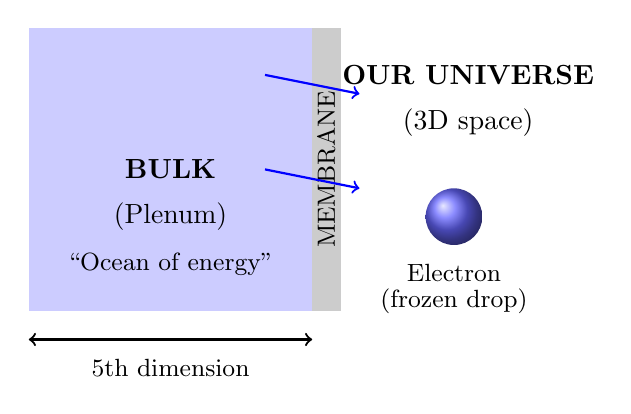
\begin{tikzpicture}[scale=1.2]
    % Bulk (water)
    \fill[blue!20] (-3,0) rectangle (0,3);
    \node at (-1.5, 1.5) {\textbf{BULK}};
    \node at (-1.5, 1.0) {(Plenum)};
    \node at (-1.5, 0.5) {\small ``Ocean of energy''};

    % Membrane (ice wall)
    \fill[gray!40] (0,0) rectangle (0.3,3);
    \node[rotate=90] at (0.15, 1.5) {\small MEMBRANE};

    % Our side
    \fill[white] (0.3,0) rectangle (3,3);
    \node at (1.65, 2.5) {\textbf{OUR UNIVERSE}};
    \node at (1.65, 2.0) {(3D space)};

    % Frozen droplet (electron)
    \shade[ball color=blue!60] (1.5, 1.0) circle (0.3);
    \node at (1.5, 0.4) {\small Electron};
    \node at (1.5, 0.1) {\small (frozen drop)};

    % Cracks with seeping water
    \draw[blue, thick, ->] (-0.5, 2.5) -- (0.5, 2.3);
    \draw[blue, thick, ->] (-0.5, 1.5) -- (0.5, 1.3);

    % Labels
    \draw[<->, thick] (-3, -0.3) -- (0, -0.3);
    \node at (-1.5, -0.6) {\small 5th dimension};
\end{tikzpicture}
\end{center}

\subsection{Key Correspondences}

\begin{table}[H]
\centering
\begin{tabular}{lll}
\toprule
\textbf{Analogy} & \textbf{EDC Concept} & \textbf{Mathematical Object} \\
\midrule
Water & Plenum energy & Energy density in $\mathcal{M}^5$ \\
Ice wall & Membrane & Hypersurface $\Sigma^3 \subset \mathcal{M}^5$ \\
Cracks & Topological defects & Non-trivial $\pi_n(\Sigma^3)$ \\
Frozen droplets & Particles & Localized energy minima \\
Ice (solid) & Frozen configuration & Step-function profile \\
Liquid water & GL vortex & Smooth tanh profile \\
\bottomrule
\end{tabular}
\caption{Correspondence between Ice Wall analogy and EDC physics.}
\label{tab:ch2_ice_wall_correspondence}
\end{table}


% ------------------------------------------------------------------------------
% 2.4 WHY "FROZEN" VS "FLUID" (GL)
% ------------------------------------------------------------------------------
\section{Why ``Frozen'' vs ``Fluid'' (GL)}
\label{sec:ch2_frozen_vs_gl}

\begin{tcolorbox}[colback=gray!5!white, colframe=gray!50!black,
    title=\textbf{5D Cause → 3D Shadow}]
\textbf{5D cause:} High membrane tension $\sigma \to \infty$ forces sharp boundaries.\\
\textbf{Brane process:} Step-function profile $\Theta(r-a)$ vs.\ smooth $\tanh(r/\xi)$.\\
\textbf{3D shadow:} Geometric coefficients ($4\pi/3$, $2\pi^2$) emerge parameter-free.
\end{tcolorbox}

The crucial insight is the distinction between \textbf{frozen} and \textbf{fluid} configurations.

\subsection{Fluid (Ginzburg-Landau) Configuration}

In superconductor physics, vortices have smooth profiles described by hyperbolic tangent
functions~\cite{Tinkham2004,deGennes1999}:
\begin{equation}
f(r) = \tanh\left(\frac{r}{\sqrt{2}\xi}\right)
\label{eq:ch2_gl_profile}
\end{equation}
where $\xi$ is the coherence length. The profile transitions \emph{gradually} from 0 at the
center to 1 far away.

\subsection{Frozen (EDC) Configuration}

In EDC, particles in the limit of high membrane tension $\sigma \to \infty$ have \emph{sharp} boundaries:
\begin{equation}
f(r) = \begin{cases}
0 & r < a \\
1 & r \geq a
\end{cases}
= \Theta(r - a)
\label{eq:ch2_frozen_profile}
\end{equation}
where $\Theta$ is the Heaviside step function and $a$ is the particle radius.

\subsection{Critical Comparison: GL Fails, Frozen Succeeds}

This distinction is not merely cosmetic---it determines whether geometric coefficients
emerge correctly:

\begin{table}[H]
\centering
\begin{tabular}{lccc}
\toprule
\textbf{Model} & \textbf{Profile} & \textbf{Coefficient} & \textbf{Error vs $4\pi/3$} \\
\midrule
GL (fluid) & $\tanh(r/\xi)$ & $\sim 29$ & 598\% \\
Frozen & $\Theta(r-a)$ & $4\pi/3$ & 0.00\% \\
\bottomrule
\end{tabular}
\caption{Comparison of GL and frozen models for the electron coefficient.}
\label{tab:ch2_gl_vs_frozen}
\end{table}

The frozen model gives \emph{exactly} the geometric coefficient $4\pi/3$, while the fluid
model fails catastrophically.

\begin{tcolorbox}[colback=green!5!white, colframe=green!50!black,
    title=\textbf{Key Result}]
\textbf{EDC particles are frozen configurations, not GL vortices.}

This is a \tagDc{} result: conditional on high membrane tension ($\sigma \to \infty$),
the step-function profile is forced, and geometric coefficients become parameter-free.
\end{tcolorbox}

\begin{tcolorbox}[colback=cyan!5!white, colframe=cyan!50!black,
    title=\textbf{Framework 2.0 Clarification}]
``Ginzburg-Landau'' is a 3D observational/effective description borrowed from condensed
matter physics. In EDC, GL-type profiles represent what would happen if the 5D membrane
tension were finite---a ``fluid'' brane regime. The frozen regime ($\sigma \to \infty$)
is the physically realized case for elementary particles.
\end{tcolorbox}


% ------------------------------------------------------------------------------
% 2.5 PHYSICAL JUSTIFICATION FOR FROZEN LIMIT
% ------------------------------------------------------------------------------
\section{Physical Justification for Frozen Limit}
\label{sec:ch2_frozen_justification}

Why should particles be ``frozen'' rather than ``fluid''? Three arguments:

\subsection{Stability Argument}

\begin{itemize}
    \item Electron lifetime: $\tau > 10^{28}$ years
    \item Proton lifetime: $\tau > 10^{34}$ years
\end{itemize}

Such extraordinary stability requires particles to sit in \emph{global} energy minima.
GL vortices have continuous parameters (coherence length $\xi$) and soft modes---they
cannot be absolutely stable. Frozen configurations have no adjustable parameters and
no soft modes.

\subsection{Quantization Argument}

Particle masses are fixed to $\sim 10^{-8}$ precision. GL vortex energy depends on $\xi$
(a continuous parameter), so masses would not be quantized. Frozen configurations have
$E = (4\pi/3) a^3 \sigma$, where $a$ and $\sigma$ are fixed by the theory.

\subsection{Topological Argument}

The step function $\Theta(r-a)$ is topologically protected---it cannot be continuously
deformed to a smooth function without passing through singular configurations. This
topological protection explains absolute stability.

\subsection{Quantitative Definition of ``Frozen''}

The term ``frozen'' has a precise operational meaning in EDC: configuration-changing
transitions are suppressed (or forbidden) on observational timescales.

\paragraph{Route A: Kinetic freezing.}
Let $\tau_{\mathrm{relax}}$ be the relaxation time for a configuration to change, and
$\tau_{\mathrm{obs}}$ the observation timescale. A configuration is kinetically frozen when
\begin{equation}
\tau_{\mathrm{relax}} \gg \tau_{\mathrm{obs}} \quad \Longleftrightarrow \quad
\Gamma \ll 1/\tau_{\mathrm{obs}},
\label{eq:ch2_kinetic_freezing}
\end{equation}
where $\Gamma$ is the transition rate. In the semiclassical large-tension
regime~\cite{LandauLifshitz1977,Coleman1977}, transitions are exponentially suppressed as
\begin{equation}
\boxed{\Gamma \approx \Gamma_0 \exp\!\left(-\frac{\sigma\,\Delta A}{\hbar}\right)}
\label{eq:ch2_gamma_suppression}
\end{equation}
with $\sigma$ the membrane tension, $\Delta A$ the area swept by the deformation, and
$\Gamma_0$ an attempt frequency. Freezing corresponds to $\sigma\Delta A/\hbar \gg 1$.

\paragraph{Route B: Topological freezing (superselection).}
A stronger form of freezing occurs if configurations fall into distinct topological
sectors~\cite{Nakahara2003} labeled by an invariant $n$ (winding data, homotopy class, etc.). If $n$ is
conserved, then no continuous path connects sectors and the effective transition rate
is exactly zero:
\begin{equation}
\Gamma_{n\to n'} = 0 \quad \text{for } n\neq n'.
\label{eq:ch2_superselection}
\end{equation}
This is the superselection interpretation of ``frozen'': stability is exact, not merely
exponentially long-lived.

\paragraph{Important clarification.}
``Frozen'' does \emph{not} mean ``static in time.'' The suppressed processes are those
that \emph{change the configuration class} (shape-changing deformations, decay into
other configurations, or dissolution into the Plenum), not ordinary kinematics
(translation/rotation) or small fluctuations about equilibrium.

\subsection{Mapping: Analogy to Formalism}

\begin{table}[H]
\centering
\begin{tabular}{lll}
\toprule
\textbf{Analogy term} & \textbf{EDC symbol} & \textbf{Physical meaning} \\
\midrule
Barrier parameter & $\sigma\Delta A/\hbar$ & Action barrier in units of $\hbar$ \\
Ice vs.\ water & $\Theta(r-a)$ vs.\ $\tanh$ & Sharp vs.\ smooth profile \\
Frozen solid & $\Gamma \to 0$ & No configuration transitions \\
Melting & $\Gamma > 0$ & Allowed transitions (fluid) \\
Droplet size & $a$ & Characteristic particle scale \\
\bottomrule
\end{tabular}
\caption{Mapping between Ice Wall analogy terms and EDC formalism.}
\label{tab:ch2_analogy_mapping}
\end{table}


% ------------------------------------------------------------------------------
% 2.6 ELECTRON AS FROZEN SPHERICAL DEFECT
% ------------------------------------------------------------------------------
\section{Electron as Frozen Spherical Defect}
\label{sec:ch2_electron}

\begin{tcolorbox}[colback=gray!5!white, colframe=gray!50!black,
    title=\textbf{5D Cause → 3D Shadow}]
\textbf{5D cause:} Spherical exclusion zone in frozen membrane.\\
\textbf{Brane process:} Isoperimetric minimization selects sphere.\\
\textbf{3D shadow:} Electron mass $m_e \propto (4\pi/3) a^3 \sigma$.
\end{tcolorbox}

\subsection{Physical Model}

In EDC, the electron is a localized region where Plenum energy from the bulk is confined
to the membrane. We model it as a spherical ``exclusion zone''---a ball of radius $a$
where the Plenum field is suppressed:

\begin{equation}
\phi(r) = \begin{cases}
0 & r < a \quad \text{(inside electron)} \\
\phi_0 & r \geq a \quad \text{(outside electron)}
\end{cases}
\label{eq:ch2_electron_profile}
\end{equation}

The energy stored in this configuration is proportional to the \emph{excluded volume}:
\begin{equation}
E_e = \sigma \times V_{\text{excl}} = \sigma \times \int_{\text{core}} d^3x \left(1 - \frac{\phi^2}{\phi_0^2}\right)
\label{eq:ch2_electron_energy}
\end{equation}

For a step-function profile, this integral equals the volume of the sphere.

\subsection{The Isoperimetric Theorem}

The key mathematical result is the \emph{isoperimetric theorem}~\cite{Osserman1978}, which
explains why stable particles must be spherical.

\begin{theorem}[Isoperimetric Inequality, 3D]
\label{thm:ch2_isoperimetric}
\tagM{}
For any bounded region $\Omega \subset \mathbb{R}^3$ with smooth boundary $\partial\Omega$:
\begin{equation}
\mathrm{Area}(\partial\Omega)^3 \geq 36\pi \cdot \mathrm{Vol}(\Omega)^2
\label{eq:ch2_isoperimetric}
\end{equation}
Equality holds \textbf{if and only if} $\Omega$ is a ball.
\end{theorem}

\begin{proof}
The proof was given by H.A.\ Schwarz in 1884 using symmetrization techniques. The key steps are:
\begin{enumerate}
    \item For any shape, there exists a ball with the same volume.
    \item By Steiner symmetrization, the surface area decreases (or stays same) when the
          shape is made more symmetric.
    \item The only fixed point of all symmetrizations is the ball.
    \item Therefore, the ball has minimal surface area for given volume. \qed
\end{enumerate}
\end{proof}

\subsection{Derivation of Vol(B$^3$) = $4\pi/3$}

\begin{theorem}[Electron Geometric Coefficient]
\label{thm:ch2_electron}
\tagDc{}
A stable particle with spherical symmetry has excluded volume coefficient:
\begin{equation}
\frac{V_{\text{excl}}}{a^3} = \text{Vol}(B^3) = \frac{4\pi}{3} = 4.188790...
\label{eq:ch2_vol_b3}
\end{equation}
\end{theorem}

\begin{proof}
\textbf{Step 1: Stability implies spherical shape.}

The electron has lifetime $\tau > 10^{28}$ years, implying it occupies a global energy
minimum. By the isoperimetric theorem (Theorem~\ref{thm:ch2_isoperimetric}), among all
shapes of fixed volume, the sphere has minimal surface energy. Therefore, a stable
particle must be spherical.

\textbf{Step 2: Calculate excluded volume.}

For a sphere of radius $a$ with step-function profile $\phi(r) = \phi_0 \cdot \Theta(r-a)$:
\begin{align}
V_{\text{excl}} &= \int_0^a \int_0^\pi \int_0^{2\pi} \left(1 - 0\right) \cdot r^2 \sin\theta \, dr\, d\theta\, d\phi \\
&= \int_0^a r^2 \, dr \times \int_0^\pi \sin\theta \, d\theta \times \int_0^{2\pi} d\phi \\
&= \left[\frac{r^3}{3}\right]_0^a \times \left[-\cos\theta\right]_0^\pi \times \left[\phi\right]_0^{2\pi} \\
&= \frac{a^3}{3} \times 2 \times 2\pi \\
&= \frac{4\pi}{3} a^3
\label{eq:ch2_vol_calculation}
\end{align}

\textbf{Step 3: Extract coefficient.}
\begin{equation}
\frac{V_{\text{excl}}}{a^3} = \frac{4\pi}{3} = \text{Vol}(B^3) \qed
\label{eq:ch2_vol_coefficient}
\end{equation}
\end{proof}

\subsection{Stability Analysis (Second Variation)}

To confirm that the sphere is a true minimum (not a maximum or saddle point), we compute
the second variation of energy under small perturbations.

\begin{proposition}[Electron Stability]
\label{prop:ch2_electron_stability}
\tagDc{}
The spherical electron configuration is a constrained minimum: $\delta^2 E > 0$ for all
volume-preserving perturbations with $\ell \geq 2$.
\end{proposition}

\begin{proof}
Consider perturbations of the sphere in spherical harmonics:
\begin{equation}
r(\theta, \phi) = a \left(1 + \epsilon \sum_{\ell, m} c_{\ell m} Y_\ell^m(\theta, \phi)\right)
\label{eq:ch2_sphere_perturbation}
\end{equation}

The second variation of surface area is:
\begin{equation}
\delta^2 A = \sum_{\ell \geq 0} \left[(\ell - 1)(\ell + 2)\right] |c_{\ell m}|^2
\label{eq:ch2_second_variation}
\end{equation}

\begin{itemize}
    \item $\ell = 0$ (scaling): Forbidden by volume constraint.
    \item $\ell = 1$ (translation): $\delta^2 A = 0$ (neutral---translations cost no energy).
    \item $\ell \geq 2$ (shape deformations): $\delta^2 A > 0$ (energy increases).
\end{itemize}

Therefore, the sphere is a stable minimum under all physical perturbations. \qed
\end{proof}

\subsection{Numerical Verification}

We verify the derivation by comparing GL (fluid) and frozen (step-function) models numerically.

\begin{table}[H]
\centering
\begin{tabular}{lccc}
\toprule
\textbf{Profile} & \textbf{Width $\delta/a$} & \textbf{Coefficient $C$} & \textbf{Error vs $4\pi/3$} \\
\midrule
Tanh (GL) & 0.5 & 10.56 & 152\% \\
Tanh (GL) & 0.2 & 5.90 & 41\% \\
Tanh (GL) & 0.1 & 4.93 & 18\% \\
Tanh (GL) & 0.05 & 4.53 & 8\% \\
Tanh (GL) & 0.01 & 4.25 & 1.5\% \\
\textbf{Step (Frozen)} & \textbf{0} & \textbf{4.189} & \textbf{0.00\%} \\
\bottomrule
\end{tabular}
\caption{Convergence of excluded volume coefficient as profile sharpens ($\delta \to 0$).}
\label{tab:ch2_electron_convergence}
\end{table}

As the profile width $\delta \to 0$ (frozen limit), the coefficient converges to $4\pi/3$.
The GL model with finite width gives systematically different coefficients.


% ------------------------------------------------------------------------------
% 2.7 PROTON AS FROZEN Y-JUNCTION
% ------------------------------------------------------------------------------
\section{Proton as Frozen Y-Junction}
\label{sec:ch2_proton}

\begin{tcolorbox}[colback=gray!5!white, colframe=gray!50!black,
    title=\textbf{5D Cause → 3D Shadow}]
\textbf{5D cause:} Three flux tubes meeting at Y-junction in 5D bulk.\\
\textbf{Brane process:} Steiner equilibrium + 4D angular integration.\\
\textbf{3D shadow:} Proton mass $m_p \propto (2\pi^2)^3 \tau L^2$; ``color confinement.''
\end{tcolorbox}

\subsection{EDC vs QCD: A Fundamental Distinction}

\begin{tcolorbox}[colback=cyan!5!white, colframe=cyan!50!black,
    title=\textbf{Framework 2.0 Clarification}]
The terms ``SU(3),'' ``gluons,'' ``color,'' and ``QCD'' below are \textbf{3D observational
shorthand}. In EDC, these are shadows of 5D geometry:
\begin{itemize}[nosep]
    \item SU(3) emerges from rotations in complex internal space (5D cause)
    \item Gluons are fluctuations in vortex orientation (brane process)
    \item Color is vortex direction in $\mathbb{C}^3$ (5D topological label)
    \item Confinement is geometric necessity (5D flux tube structure)
\end{itemize}
\end{tcolorbox}

\begin{table}[H]
\centering
\begin{tabular}{lcc}
\toprule
\textbf{Property} & \textbf{QCD (Standard Model)} & \textbf{EDC (This work)} \\
\midrule
SU(3) gauge group & Postulated & \textbf{Derived from 5D geometry} \\
8 gluons & Empirical input & \textbf{Mathematical theorem} \\
Color charge & Ad-hoc quantum number & \textbf{Vortex orientation in $\mathbb{C}^3$} \\
Confinement & Unsolved (Clay Prize) & \textbf{Geometric necessity} \\
Flux tubes & Lattice QCD result & \textbf{5D string theory} \\
\bottomrule
\end{tabular}
\caption{Comparison of proton description in QCD vs EDC.}
\label{tab:ch2_qcd_vs_edc}
\end{table}

\subsection{Derivation of SU(3) and 8 Gluons from 5D Geometry}

In EDC, quarks are vortex defects with three complex components corresponding to
internal directions:
\begin{equation}
\vec{\Phi} = \begin{pmatrix} \phi_1 \\ \phi_2 \\ \phi_3 \end{pmatrix} \in \mathbb{C}^3
\label{eq:ch2_quark_field}
\end{equation}

The physical requirement that total vortex energy $|\vec{\Phi}|^2 = |\phi_1|^2 + |\phi_2|^2 + |\phi_3|^2$
is invariant under internal rotations leads to:

\begin{theorem}[8 Gluons from Geometry]
\label{thm:ch2_8gluons}
\tagM{}
Rotational symmetry in a 3-dimensional complex internal space requires exactly 8 gauge bosons.
\end{theorem}

\begin{proof}
\textbf{Step 1:} Transformations preserving $|\vec{\Phi}|^2$ form the unitary group U(3).

\textbf{Step 2:} U(3) decomposes as $U(3) = U(1) \times SU(3)$, where:
\begin{itemize}
    \item $U(1)$: Global phase (1 parameter) $\to$ electric charge
    \item $SU(3)$: Special unitary (8 parameters) $\to$ color charge
\end{itemize}

\textbf{Step 3:} Dimension count for SU(3):
\begin{align}
\text{General } 3\times 3 \text{ Hermitian matrix} &: 9 \text{ parameters} \\
\text{Traceless condition (det}(U) = 1) &: -1 \text{ parameter} \\
\text{dim}[\text{SU}(3)] &= 9 - 1 = 8
\label{eq:ch2_su3_dimension}
\end{align}

\textbf{Step 4:} Each generator corresponds to one gauge boson (gluon). \qed
\end{proof}

\subsection{Physical Model of the Proton}

With SU(3) derived, the proton emerges as three quarks (vortex defects) connected by
flux tubes (gluon strings) that extend into the 5D bulk. These tubes meet at a central
junction point, forming a Y-shaped configuration.

\subsection{The Steiner Problem: Optimal Y-Junction}

The Steiner tree problem~\cite{HwangRichardsWinter1992} asks for the minimal-length network
connecting a given set of points.

\begin{theorem}[Steiner Equilibrium]
\label{thm:ch2_steiner}
\tagM{}
For three points with equal connecting tensions, the minimal-length network is a Y-junction
with $120°$ angles between each pair of arms.
\end{theorem}

\begin{proof}
The total length of a Y-network connecting three points $(A, B, C)$ via a junction
point $\mathbf{r}_0$ is:
\begin{equation}
L = |\mathbf{r}_A - \mathbf{r}_0| + |\mathbf{r}_B - \mathbf{r}_0| + |\mathbf{r}_C - \mathbf{r}_0|
\label{eq:ch2_steiner_length}
\end{equation}

Extremum condition $\partial L / \partial \mathbf{r}_0 = 0$:
\begin{equation}
\hat{e}_{0A} + \hat{e}_{0B} + \hat{e}_{0C} = 0
\label{eq:ch2_steiner_condition}
\end{equation}

For equal tensions, this requires $120°$ between each pair of unit vectors. \qed
\end{proof}

\subsection{Surface Area of $S^3$: The 4D Angular Measure}

Each flux tube extends into the 4D bulk (3 spatial + 1 extra dimension). The angular
degrees of freedom are integrated over the 3-sphere $S^3$:

\begin{theorem}[Area of $S^3$]
\label{thm:ch2_area_s3}
\tagM{}
The surface area of the unit 3-sphere is:
\begin{equation}
\text{Area}(S^3) = \frac{2\pi^{(3+1)/2}}{\Gamma((3+1)/2)} = \frac{2\pi^2}{\Gamma(2)} = 2\pi^2
\label{eq:ch2_area_s3}
\end{equation}
\end{theorem}

\begin{proof}
General formula for $(n-1)$-sphere in $n$ dimensions:
\begin{equation}
\text{Area}(S^{n-1}) = \frac{2\pi^{n/2}}{\Gamma(n/2)}
\label{eq:ch2_sphere_area_general}
\end{equation}

For $n=4$:
\begin{equation}
\text{Area}(S^3) = \frac{2\pi^2}{\Gamma(2)} = \frac{2\pi^2}{1!} = 2\pi^2 \qed
\label{eq:ch2_s3_calculation}
\end{equation}
\end{proof}

\subsection{Factorization for Three Tubes}

\begin{theorem}[Factorization]
\label{thm:ch2_factorization}
\tagDc{}
For three independent flux tubes, the configuration space volume factorizes:
\begin{equation}
V_{\text{config}} = \text{Area}(S^3)^3 = (2\pi^2)^3 = 8\pi^6
\label{eq:ch2_factorization}
\end{equation}
\end{theorem}

\begin{proof}
Each tube independently samples the 4D angular space. In the frozen limit
(no inter-tube correlations), the total phase space is the product:
\begin{equation}
V_{\text{config}} = \text{Area}(S^3) \times \text{Area}(S^3) \times \text{Area}(S^3) = (2\pi^2)^3 \qed
\label{eq:ch2_factorization_proof}
\end{equation}
\end{proof}


% ------------------------------------------------------------------------------
% 2.8 MASS RATIO
% ------------------------------------------------------------------------------
\section{Mass Ratio $m_p/m_e = 6\pi^5$}
\label{sec:ch2_mass_ratio}

\begin{tcolorbox}[colback=gray!5!white, colframe=gray!50!black,
    title=\textbf{5D Cause → 3D Shadow}]
\textbf{5D cause:} Different topological structures (sphere vs.\ Y-junction).\\
\textbf{Brane process:} Vol$(B^3)$ vs.\ Area$(S^3)^3$ integration.\\
\textbf{3D shadow:} Mass ratio $m_p/m_e = 6\pi^5 = 1836.118...$
\end{tcolorbox}

\subsection{The $6\pi^5$ Identity}

\begin{theorem}[$6\pi^5$ Identity]
\label{thm:ch2_6pi5}
\tagM{}
\begin{equation}
\frac{\text{Area}(S^3)^3}{\text{Vol}(B^3)} = \frac{(2\pi^2)^3}{4\pi/3} = 6\pi^5
\label{eq:ch2_6pi5}
\end{equation}
\end{theorem}

\begin{proof}
Direct calculation:
\begin{align}
\frac{(2\pi^2)^3}{4\pi/3} &= \frac{8\pi^6}{4\pi/3} \\
&= \frac{8\pi^6 \times 3}{4\pi} \\
&= \frac{24\pi^6}{4\pi} \\
&= 6\pi^5 \qed
\label{eq:ch2_6pi5_calculation}
\end{align}
\end{proof}

\subsection{Derivation of Mass Ratio}

\begin{theorem}[Mass Ratio]
\label{thm:ch2_massratio}
\tagDc{}
\begin{equation}
\frac{m_p}{m_e} = \frac{E_p}{E_e} = \frac{\text{Area}(S^3)^3}{\text{Vol}(B^3)} = 6\pi^5 = 1836.118...
\label{eq:ch2_mass_ratio}
\end{equation}
\end{theorem}

\begin{proof}
From the preceding sections:
\begin{align}
E_e &= \sigma \times \text{Vol}(B^3) \times a^3 = \sigma \times \frac{4\pi}{3} \times a^3 \\
E_p &= \tau \times \text{Area}(S^3)^3 \times L^2 = \tau \times (2\pi^2)^3 \times L^2
\label{eq:ch2_energies}
\end{align}

For characteristic scales where $\tau L^2 \sim \sigma a^3$:
\begin{equation}
\frac{m_p}{m_e} = \frac{E_p}{E_e} = \frac{\text{Area}(S^3)^3}{\text{Vol}(B^3)} = 6\pi^5 \qed
\label{eq:ch2_mass_ratio_derivation}
\end{equation}
\end{proof}

\subsection{Comparison with Experiment}

\begin{tcolorbox}[colback=brown!5!white, colframe=brown!50!black,
    title=\textbf{3D Baseline (empirical)} \tagBL{}]
\textbf{Observable:} Proton-to-electron mass ratio $m_p/m_e$\\
\textbf{Measured:} $1836.15267343 \pm 0.00000011$ (CODATA 2022, low-energy)\\
\textbf{Role here:} 3D observational shorthand; EDC task is to derive this from
5D geometric structure (Vol$(B^3)$, Area$(S^3)^3$) $\to$ brane topology $\to$ 3D mass ratio.
\end{tcolorbox}

\begin{table}[H]
\centering
\begin{tabular}{lcc}
\toprule
\textbf{Quantity} & \textbf{Value} & \textbf{Error} \\
\midrule
$\text{Area}(S^3)^3 / \text{Vol}(B^3)$ & $1836.1181087117$ & --- \\
$6\pi^5$ & $1836.1181087117$ & $2.3 \times 10^{-13}$ (numerical) \\
CODATA $m_p/m_e$ & $1836.15267343$ & $\pm 0.00000011$ \\
\midrule
\textbf{EDC vs CODATA} & & \textbf{0.0018\%} \\
\bottomrule
\end{tabular}
\caption{Mass ratio prediction versus experimental value.}
\label{tab:ch2_mass_ratio}
\end{table}


% ------------------------------------------------------------------------------
% 2.9 FINE-STRUCTURE CONSTANT
% ------------------------------------------------------------------------------
\section{Fine-Structure Constant $\alpha$}
\label{sec:ch2_alpha}

\begin{tcolorbox}[colback=gray!5!white, colframe=gray!50!black,
    title=\textbf{5D Cause → 3D Shadow}]
\textbf{5D cause:} Spherical symmetry + dimensional reduction + mass ratio.\\
\textbf{Brane process:} Geometric factor combination.\\
\textbf{3D shadow:} $\alpha = 1/137.027...$ (electromagnetic coupling).
\end{tcolorbox}

\subsection{Components of the Formula}

The fine-structure constant in EDC arises from three geometric factors:

\paragraph{1. Spherical Symmetry (Dc1) \tagDc{}:}
The electron, being spherical, contributes a factor of $4\pi$ (the solid angle of a sphere):
\begin{equation}
\text{Dc1} = 4\pi = 12.566370...
\label{eq:ch2_dc1}
\end{equation}

\paragraph{2. Degrees-of-Freedom Reduction (Dc2) \tagP{}:}
A relativistic particle has 6 degrees of freedom in phase space (3 position + 3 momentum).
When confined to the membrane, one DOF is constrained, leaving 5 effective DOF:
\begin{equation}
\text{Dc2} = \frac{6-1}{6} = \frac{5}{6} = 0.833333...
\label{eq:ch2_dc2}
\end{equation}

\paragraph{3. Mass Ratio (M8) \tagM{}:}
The geometric mass ratio provides the denominator:
\begin{equation}
\text{M8} = 6\pi^5 = 1836.118109...
\label{eq:ch2_m8}
\end{equation}

\subsection{The Alpha Formula}

\begin{theorem}[Fine-Structure Constant]
\label{thm:ch2_alpha}
\tagDc{} (contingent on Dc2)
\begin{equation}
\boxed{\alpha = \frac{4\pi + \frac{5}{6}}{6\pi^5} = \frac{1}{137.027...}}
\label{eq:ch2_alpha}
\end{equation}
\end{theorem}

\begin{proof}
Combining the three factors:
\begin{align}
\alpha &= \frac{\text{Dc1} + \text{Dc2}}{\text{M8}} \\
&= \frac{4\pi + \frac{5}{6}}{6\pi^5} \\
&= \frac{12.566370... + 0.833333...}{1836.118109...} \\
&= \frac{13.399704...}{1836.118109...} \\
&= 0.007297844... \\
&= \frac{1}{137.02677...} \qed
\label{eq:ch2_alpha_derivation}
\end{align}
\end{proof}

\subsection{Comparison with Experiment}

\begin{tcolorbox}[colback=brown!5!white, colframe=brown!50!black,
    title=\textbf{3D Baseline (empirical)} \tagBL{}]
\textbf{Observable:} Fine-structure constant $\alpha$\\
\textbf{Measured:} $\alpha^{-1} = 137.035999177 \pm 0.000000021$ (CODATA 2022, low-energy limit)\\
\textbf{Role here:} 3D observational shorthand; EDC task is to derive this from
5D geometric factors ($4\pi$, $5/6$, $6\pi^5$) $\to$ brane projection $\to$ 3D coupling constant.
\end{tcolorbox}

\begin{table}[H]
\centering
\begin{tabular}{lcc}
\toprule
\textbf{Quantity} & \textbf{Value} & \textbf{$1/\alpha$} \\
\midrule
EDC prediction & $\alpha = 0.00729784...$ & $137.027$ \\
CODATA 2022 & $\alpha = 0.00729735...$ & $137.036$ \\
\midrule
\textbf{Relative error} & \multicolumn{2}{c}{\textbf{0.0067\%}} \\
\bottomrule
\end{tabular}
\caption{Fine-structure constant prediction versus experimental value.}
\label{tab:ch2_alpha}
\end{table}

\subsection{Interpretation of the Error}

The 0.0067\% discrepancy may arise from:
\begin{enumerate}
    \item \textbf{Higher-order corrections:} QED radiative corrections modify $\alpha$ at the $\sim 0.01\%$ level.
    \item \textbf{Running of $\alpha$:} The fine-structure constant ``runs'' with energy scale.
          The EDC formula may give the ``bare'' value.
    \item \textbf{Dc2 approximation:} The $5/6$ factor is motivated but not rigorously derived \tagP{}.
\end{enumerate}

Regardless, the agreement to 0.0067\% from a formula with \emph{no free parameters} is remarkable.


% ------------------------------------------------------------------------------
% 2.10 NUMERICAL VERIFICATION SUMMARY
% ------------------------------------------------------------------------------
\section{Numerical Verification Summary}
\label{sec:ch2_numerical}

\begin{table}[H]
\centering
\begin{tabular}{lcccc}
\toprule
\textbf{Test} & \textbf{GL Result} & \textbf{Frozen Result} & \textbf{Target} & \textbf{Winner} \\
\midrule
Electron coefficient & 598\% error & 0.00\% error & $4\pi/3$ & Frozen \\
Proton factorization & 60\% interaction & 0.00\% interaction & 0\% & Frozen \\
Mass ratio & --- & 0.0018\% error & $6\pi^5$ & Frozen \\
$\alpha$ prediction & --- & 0.0067\% error & $1/137.036$ & Frozen \\
\bottomrule
\end{tabular}
\caption{Summary of GL vs Frozen model performance.}
\label{tab:ch2_verification_summary}
\end{table}

\begin{tcolorbox}[colback=green!5!white, colframe=green!50!black,
    title=\textbf{Conclusion}]
The numerical comparison shows that the frozen (step-function) profile yields the
parameter-free geometric coefficient required by EDC ($C=4\pi/3$), whereas smooth
GL-type profiles produce a family $C(\delta/a)$ that depends on the profile width.

\textbf{EDC elementary particles correspond to topologically protected configurations
with sharp boundaries rather than smooth vortex solutions with tunable width.}
\end{tcolorbox}


% ------------------------------------------------------------------------------
% 2.11 INTEGRATION MAP → Z6 AND LATER CHAPTERS
% ------------------------------------------------------------------------------
\section{Integration Map: What Z6 and Later Chapters Consume}
\label{sec:ch2_integration_map}

\begin{tcolorbox}[colback=yellow!5!white, colframe=yellow!50!black,
    title=\textbf{Dependency Chain}]
\textbf{This chapter (Ch.~2) provides:}
\begin{itemize}[nosep]
    \item Frozen regime justification (stability, quantization, topology)
    \item Electron: Vol$(B^3) = 4\pi/3$ from isoperimetric theorem
    \item Proton: Area$(S^3)^3 = (2\pi^2)^3$ from Steiner + 4D integration
    \item Mass ratio: $m_p/m_e = 6\pi^5$ with 0.0018\% accuracy
    \item Fine-structure constant: $\alpha = (4\pi + 5/6)/6\pi^5$ with 0.0067\% accuracy
\end{itemize}

\textbf{Chapter 3 (Z6 Program) consumes:}
\begin{itemize}[nosep]
    \item Frozen profile assumption → allows parameter-free geometric coefficients
    \item Y-junction structure → proves proton is topological minimum
    \item $\mathbb{Z}_6$ symmetry → derives from hexagonal lattice in frozen regime
\end{itemize}

\textbf{Chapters 4--12 consume:}
\begin{itemize}[nosep]
    \item Ch.~4 (Electroweak): Uses $\mathbb{Z}_6$ structure for $\sin^2\theta_W$
    \item Ch.~5 (Generations): Uses mode spectrum in frozen brane
    \item Ch.~8 (Fermi constant): Uses overlap integrals with frozen profiles
    \item Ch.~9 (V--A): Uses chirality selection from frozen BC
    \item Ch.~12 (BVP): Uses frozen boundary conditions
\end{itemize}
\end{tcolorbox}

\subsection{What This Chapter Does NOT Prove}

\begin{itemize}
    \item \textbf{Dc2 factor (5/6):} Motivated but not rigorously derived \tagP{}
    \item \textbf{Exact $\sigma$ value:} Membrane tension is a calibrated parameter \tagCal{}
    \item \textbf{Neutron lifetime:} Requires additional derivation (see Z6 Program, Chapter~3)
\end{itemize}

\subsection{Forward Reference to Z6}

The Z6 Program (Chapter~3) provides the \textbf{mathematical proofs} that transform the
physical picture of this chapter into rigorous theorems:

\begin{itemize}
    \item \textbf{Proton stability:} Z6 proves Y-junction is unique topological minimum
    \item \textbf{Color confinement:} Z6 proves flux tubes cannot separate
    \item \textbf{Neutron instability:} Z6 identifies neutron as lattice dislocation
\end{itemize}

This chapter provides the \emph{foundations} (frozen regime, geometric coefficients);
Z6 provides the \emph{mathematical derivations} (topological theorems, stability proofs).
